A multi layer perceptron (MLP) is a simple but powerful machine learning model, which maps an input vector to an output vector by applying successive "layers" of parameterised linear transformations followed by element-wise nonlinear functions to the input vector. The parameters of the linear transformations can be learnt in such a way as to minimise a loss function appropriate to a specific dataset using gradient-based methods, with gradients being calculated using automatic differentiation. For the experiments in this section, various different types of MLPs were trained on the MNIST dataset of handwritten digits \cite{lecun2010mnist}, using a softmax cross-entropy loss function which is appropriate for multi-class classification tasks.

There are various design decisions to consider when implementing a MLP, including the choice of method used to initialise parameters in the model, and the choice of optimisation method. The parameters of the models used in this section were initialised following \cite{he2015delving}, by sampling initial weight parameters in each layer from a zero-mean Gaussian distribution whose standard deviation is equal to $\sqrt{2/n_l}$, where $n_l$ is the dimension of the input to the layer, and initialising all bias parameters to zero. This choice of standard deviation ensures that when using rectified linear unit (relu) activation functions, the outputs from each layer do not grow or shrink exponentially. For optimising MLPs, stochastic gradient descent with momentum was used following \cite{sutskever2013importance} and \cite{polyak1964some}, in which the parameters $w_t$ at time $t$ are chosen to minimise a loss function $f$ by maintaining an estimate for the momentum $b_t$ of the parameter gradients at each time step, and updating the parameters and momentum as follows (where $\mu$ and $\alpha$ are hyperparameters to be chosen):
\begin{align}
    b_t &\leftarrow \mu b_{t-1} + \frac{\partial f}{\partial w} \\
    w_t &\leftarrow w_{t-1} - \alpha b_t
\end{align}
Figure \ref{fig:mnist cpu gpu} shows the loss function against time for two different MLPs trained on MNIST for 5 epochs, with both MLPs being trained on both an Intel(R) Core(TM) i7-1065G7 CPU @ 1.30GHz and an NVIDIA GeForce MX250 GPU for comparison. The figures show the loss function decreasing over time in all four cases, with the GPU performing faster than the CPU for both models, however the speed up offered by the GPU is more significant for the larger model (figure \ref{fig:mnist larger}). In fact, the GPU is only 6.8\% slower for the larger model, despite having to perform significantly more computation, whereas the CPU is 82.2\% slower. Figure \ref{fig:mnist cpu gpu server} shows analogous results for the same two models being trained on a server with Intel(R) Xeon(R) Gold 5120 CPU @ 2.20GHz and NVIDIA TITAN V GPU, showing that the server is significantly faster in all cases (both for larger and smaller models being trained on the CPU and the GPU), with the GPU actually being marginally slower for the small model, but marginally faster for the larger model.

Figure \ref{fig:mnist parameters} shows how the learning curves and final generalisation performance of a MLP trained using gradient descent vary with respect to the momentum hyperparameter (\ref{fig:mnist momentum}), batch size (\ref{fig:mnist batch size}), number of hidden layers (\ref{fig:mnist num hidden layers}), dimension of the hidden layers (\ref{fig:mnist hidden dimension}), and hidden layer activation function (\ref{fig:mnist activation function}). Figure \ref{fig:mnist predictions} shows the predictions of a trained MLP on different unseen examples of each digit from the test set.
\begin{figure}
    \centering
    \begin{subfigure}{0.45\textwidth}
        \centering
        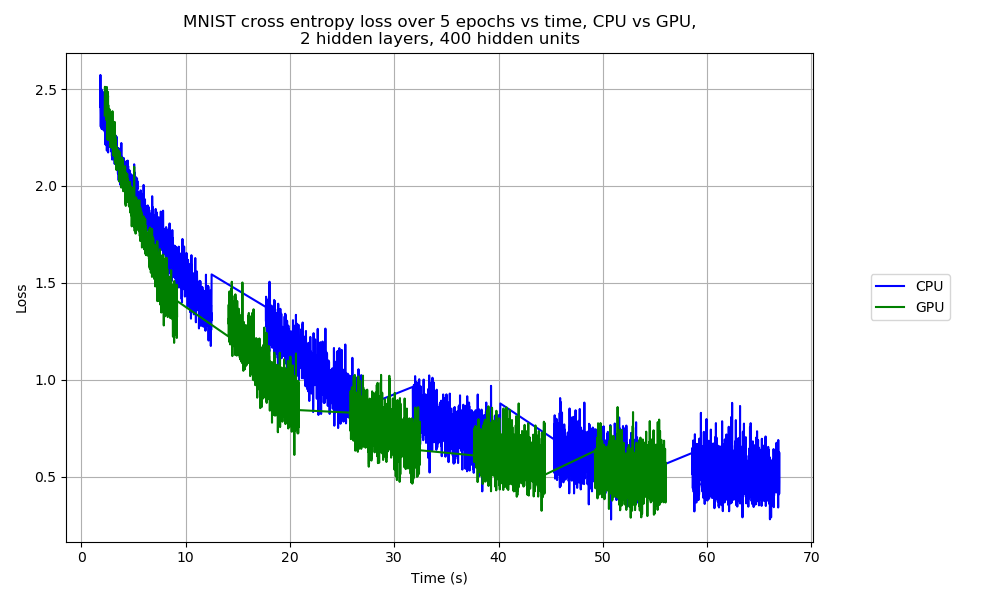
\includegraphics[width=\textwidth]{MNIST_cross_entropy_loss_over_5_epochs_vs_time,_CPU_vs_GPU,_2_hidden_layers,_400_hidden_units.png}
        \caption{Small model (2 hidden layers, 400 hidden units)}
        \label{fig:mnist small}
    \end{subfigure}
    \begin{subfigure}{0.45\textwidth}
        \centering
        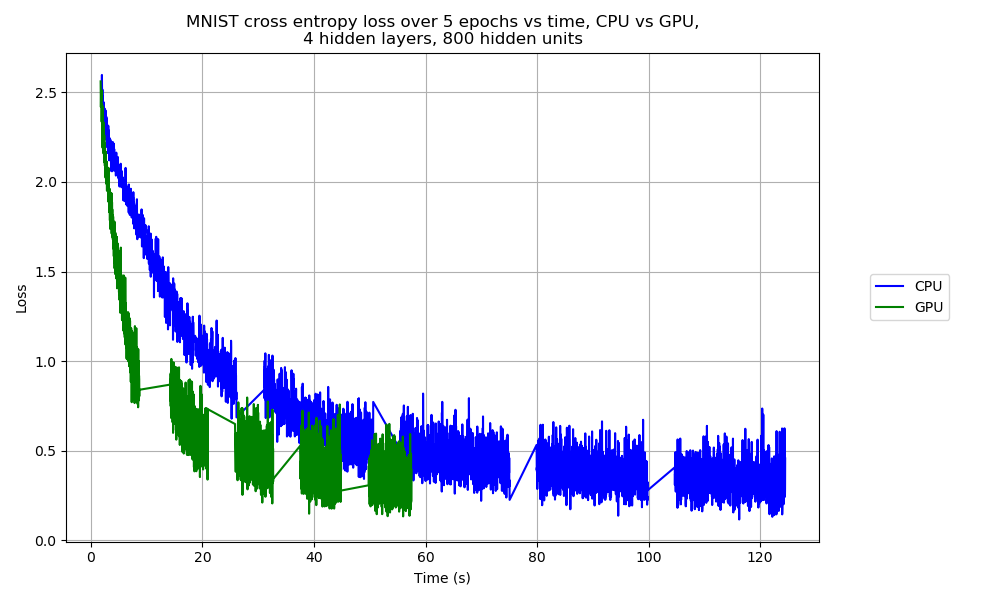
\includegraphics[width=\textwidth]{MNIST_cross_entropy_loss_over_5_epochs_vs_time,_CPU_vs_GPU,_4_hidden_layers,_800_hidden_units.png}
        \caption{Larger model (4 hidden layers, 800 hidden units)}
        \label{fig:mnist larger}
    \end{subfigure}
    \caption{Learning curves for different sized models trained on MNIST over 5 epochs, comparing training times between an Intel(R) Core(TM) i7-1065G7 CPU @ 1.30GHz and an NVIDIA GeForce MX250 GPU. Gaps in the training curves are due to evaluating test set accuracy once per epoch.}
    \label{fig:mnist cpu gpu}
\end{figure}
\begin{figure}
    \centering
    \begin{subfigure}{0.45\textwidth}
        \centering
        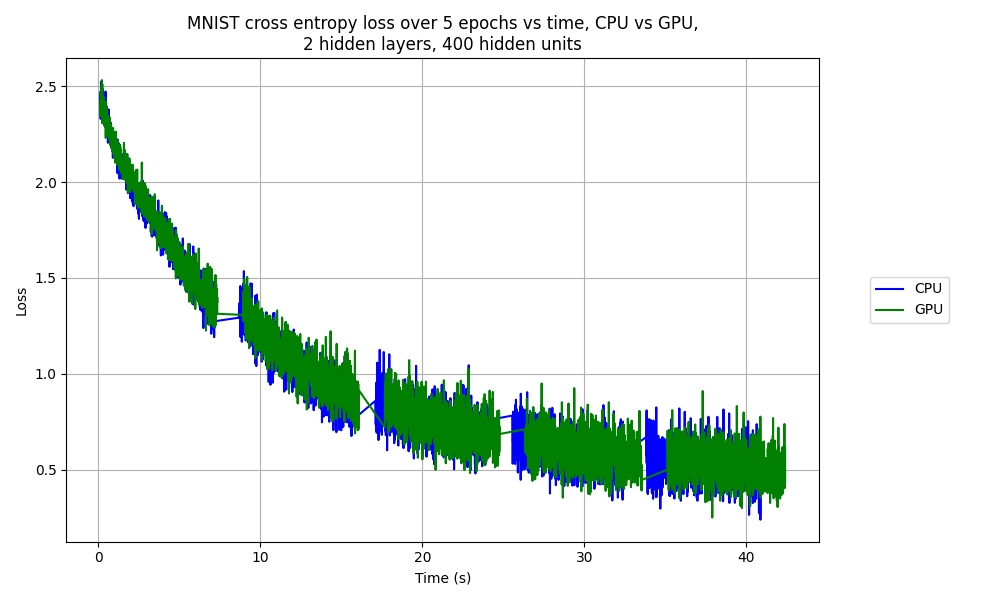
\includegraphics[width=\textwidth]{server_MNIST_cross_entropy_loss_over_5_epochs_vs_time,_CPU_vs_GPU,_2_hidden_layers,_400_hidden_units.png}
        \caption{Small model (2 hidden layers, 400 hidden units)}
        \label{fig:mnist small server}
    \end{subfigure}
    \begin{subfigure}{0.45\textwidth}
        \centering
        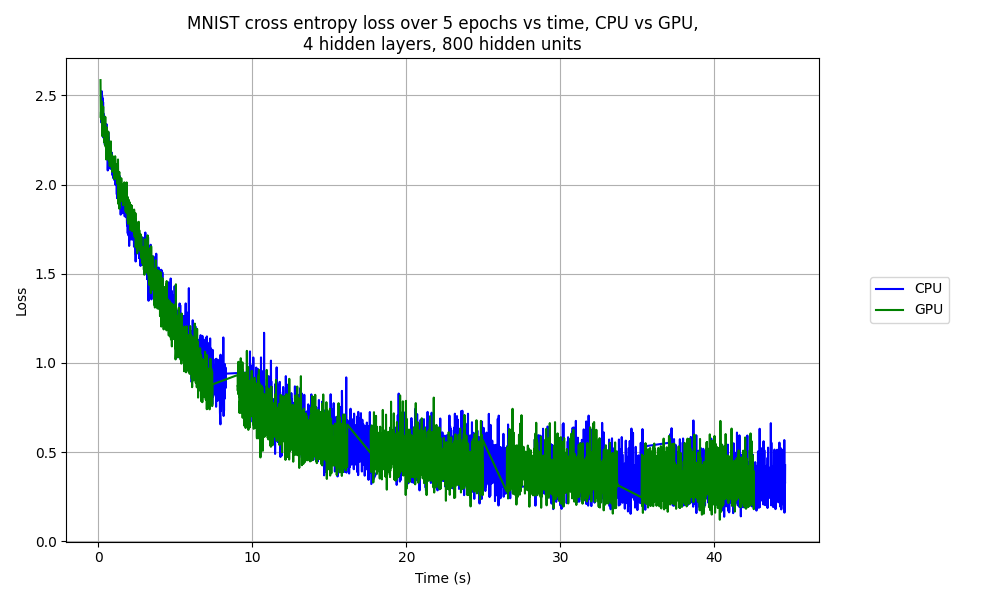
\includegraphics[width=\textwidth]{server_MNIST_cross_entropy_loss_over_5_epochs_vs_time,_CPU_vs_GPU,_4_hidden_layers,_800_hidden_units.png}
        \caption{Larger model (4 hidden layers, 800 hidden units)}
        \label{fig:mnist larger server}
    \end{subfigure}
    \caption{As for figure \ref{fig:mnist cpu gpu}, performed on a server with Intel(R) Xeon(R) Gold 5120 CPU @ 2.20GHz and NVIDIA TITAN V GPU}
    \label{fig:mnist cpu gpu server}
\end{figure}
\begin{figure}
    \centering
    \begin{subfigure}{0.45\textwidth}
        \centering
        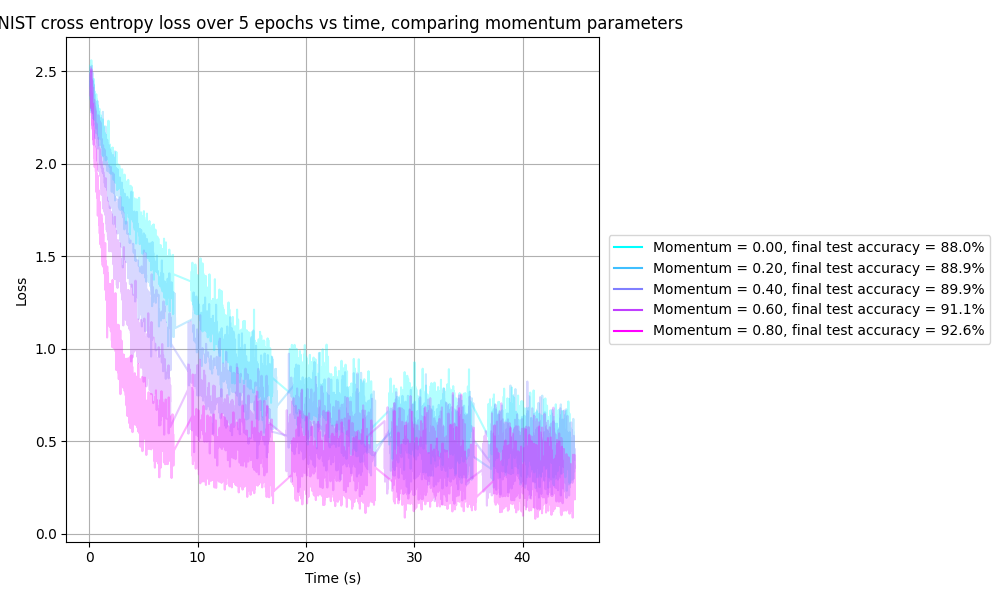
\includegraphics[width=\textwidth]{MNIST_cross_entropy_loss_over_5_epochs_vs_time,_comparing_momentum_parameters.png}
        \caption{Comparing momentum optimisation hyperparameter}
        \label{fig:mnist momentum}
    \end{subfigure}
    \begin{subfigure}{0.45\textwidth}
        \centering
        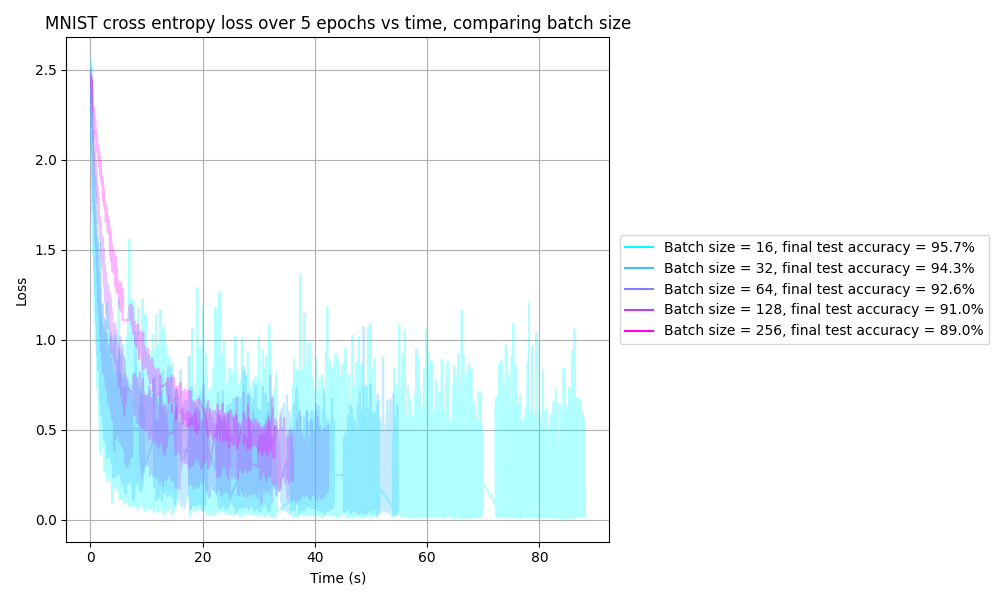
\includegraphics[width=\textwidth]{MNIST_cross_entropy_loss_over_5_epochs_vs_time,_comparing_batch_size.png}
        \caption{Comparing batch size}
        \label{fig:mnist batch size}
    \end{subfigure}
    \newline
    \begin{subfigure}{0.45\textwidth}
        \centering
        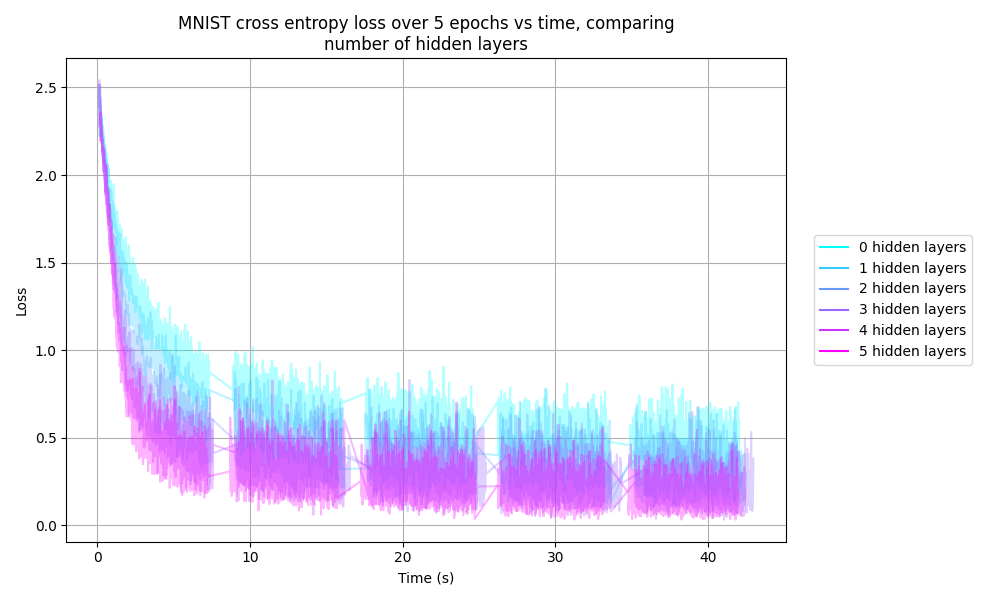
\includegraphics[width=\textwidth]{MNIST_cross_entropy_loss_over_5_epochs_vs_time,_comparing_number_of_hidden_layers.png}
        \caption{Comparing number of hidden layers}
        \label{fig:mnist num hidden layers}
    \end{subfigure}
    \begin{subfigure}{0.45\textwidth}
        \centering
        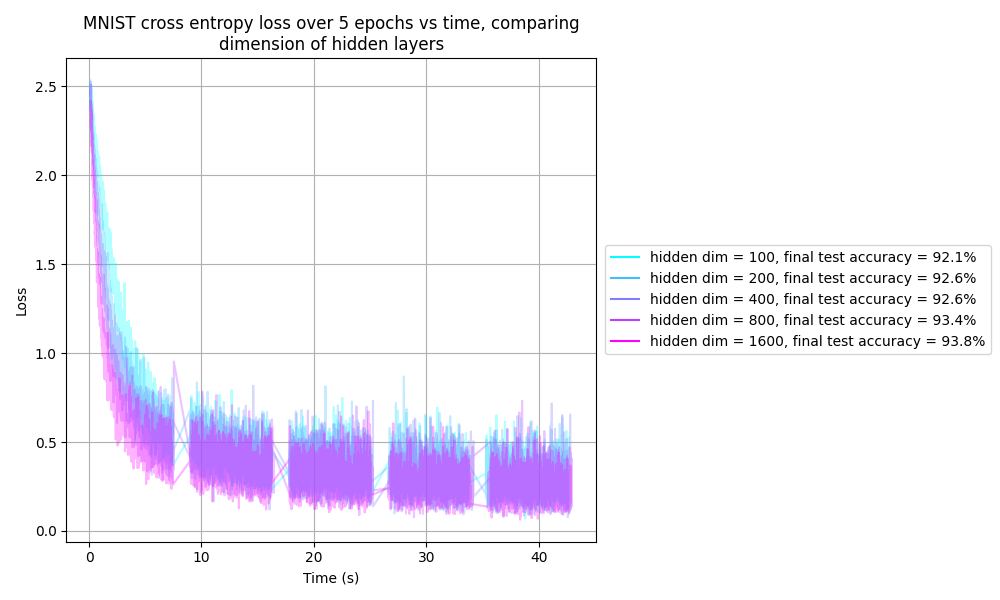
\includegraphics[width=\textwidth]{MNIST_cross_entropy_loss_over_5_epochs_vs_time,_comparing_dimension_of_hidden_layers.png}
        \caption{Comparing dimension of hidden layers}
        \label{fig:mnist hidden dimension}
    \end{subfigure}
    \newline
    \begin{subfigure}{0.45\textwidth}
        \centering
        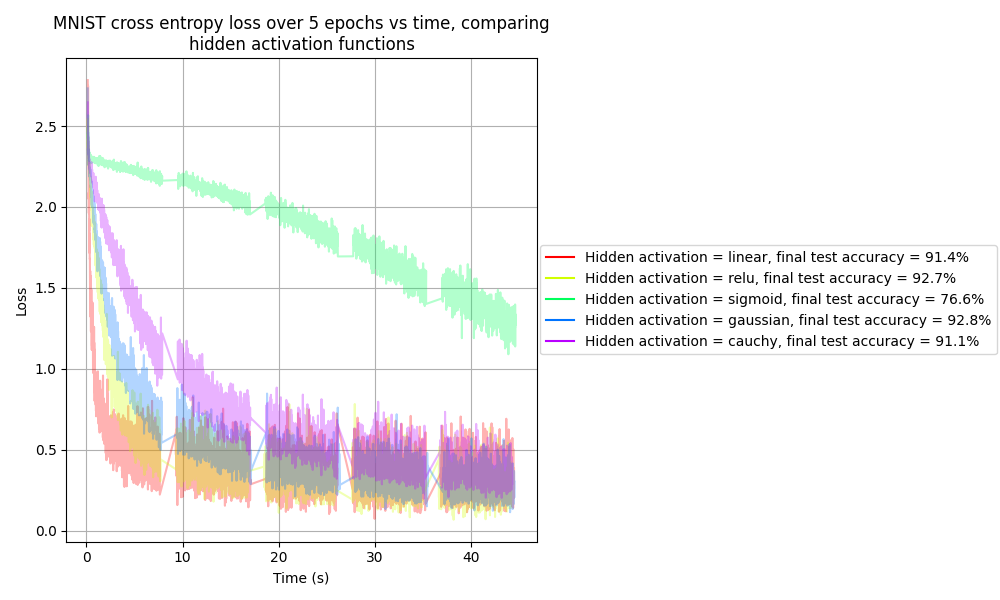
\includegraphics[width=\textwidth]{MNIST_cross_entropy_loss_over_5_epochs_vs_time,_comparing_hidden_activation_functions.png}
        \caption{Comparing hidden layer activation functions}
        \label{fig:mnist activation function}
    \end{subfigure}
    \caption{Comparing the effect of different hyperparameters on training a MLP on MNIST. Test set prediction accuracies are included in legends.}
    \label{fig:mnist parameters}
\end{figure}
\begin{figure}
    \centering
    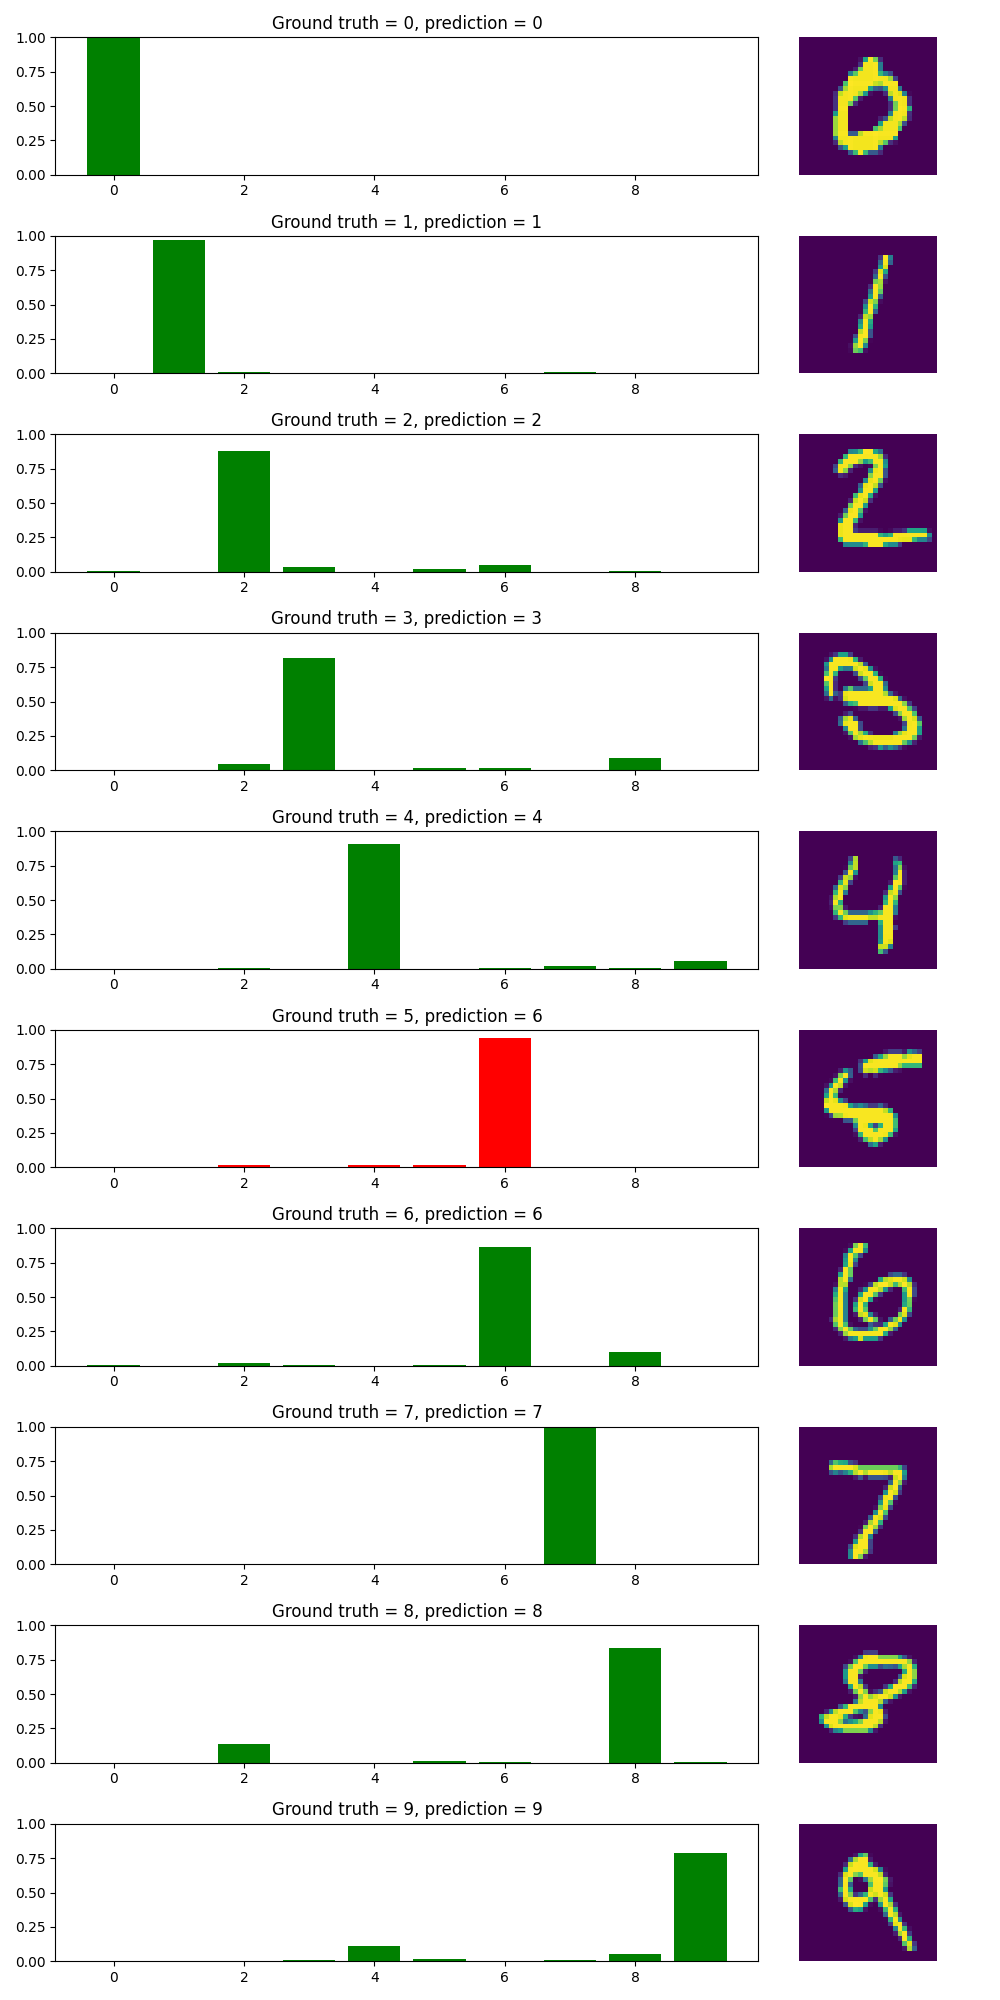
\includegraphics[width=0.6\textwidth]{Test_set_predictions.png}
    \caption{Predictions of a MLP trained on MNIST for 5 epochs on unseen examples of each digit from the test set}
    \label{fig:mnist predictions}
\end{figure}
